\documentclass[12pt,a4paper]{article}

\usepackage[margin=2.5cm]{geometry}
\usepackage[utf8]{inputenc}
\usepackage[T1]{fontenc}
\usepackage{helvet}
\renewcommand{\familydefault}{\sfdefault}
\usepackage[spanish,es-nodecimaldot]{babel}
\usepackage{graphicx}
\graphicspath{{imagenes/}}
\usepackage{float}
\usepackage{caption}
\usepackage{setspace}
\usepackage{titlesec}
\usepackage{fancyhdr}
\usepackage{ragged2e}
\usepackage{enumitem}
\usepackage[hidelinks]{hyperref}
\usepackage{xurl}

\setlength{\parindent}{1.25cm}
\setlength{\parskip}{0pt}
\setcounter{tocdepth}{2}
\setcounter{secnumdepth}{2}

\titleformat{\section}
  {\bfseries\fontsize{14}{17}\selectfont}
  {\thesection}{0.8em}{}
\titleformat{name=\section,numberless}
  {\bfseries\fontsize{14}{17}\selectfont}
  {}{0pt}{}
\titleformat{\subsection}
  {\bfseries\fontsize{12}{15}\selectfont}
  {\thesubsection}{0.8em}{}
\titlespacing*{\section}{0pt}{18pt}{10pt}
\titlespacing*{\subsection}{0pt}{14pt}{7pt}

\captionsetup{
  font={small,stretch=1.0},
  labelfont=bf,
  labelsep=period,
  justification=centering,
  singlelinecheck=false
}
\renewcommand{\figurename}{Figura}
\renewcommand{\contentsname}{Índice}
\renewcommand{\listfigurename}{Índice de imágenes}

\fancypagestyle{contenido}{
  \fancyhf{}
  \fancyhead[R]{\thepage}
  \renewcommand{\headrulewidth}{0pt}
  \renewcommand{\footrulewidth}{0pt}
}

\begin{document}

\begin{titlepage}
  \centering
  \vspace*{1.2cm}
  
\includegraphics[width=0.20\textwidth]{logo_upp.png}

  \vspace{1.0cm}
  {\bfseries\fontsize{14}{17}\selectfont Universidad Politécnica de Pachuca\par}
  \vspace{0.8cm}
  {\bfseries\fontsize{14}{17}\selectfont Desarrollo de Aplicaciones Móviles\par}
  \vspace{0.8cm}
  {\bfseries\fontsize{14}{17}\selectfont Perfil profesional con Jetpack Compose\par}
  \vspace{0.3cm}
  {\bfseries\fontsize{12}{15}\selectfont Examen Parcial 2\par}

  \vspace{1.2cm}
  {\bfseries Autor:\par}
  \vspace{0.25cm}
  Cabrera Bardales Edgar Alejandro\par
  \vspace{0.2cm}
  2531126226\par

  \vspace{0.8cm}
  {\bfseries Profesor:\par}
  \vspace{0.25cm}
  Ing. Montoya Cerro Miguel Ángel\par

  \vspace{0.8cm}
  {\bfseries Grupo:\par}
  \vspace{0.25cm}
  TIID 04-01\par

  \vfill
  Zempoala, Hidalgo, México a 06 de noviembre de 2026\par
\end{titlepage}

\pagestyle{empty}
\begingroup
\setstretch{1.15}
\tableofcontents
\clearpage
\listoffigures
\endgroup
\clearpage

\setcounter{page}{1}
\pagestyle{contenido}
\RaggedRight
\doublespacing

\section{Introducción}

En el desarrollo de aplicaciones móviles para Android, la presentación visual de una pantalla resulta importante para organizar la información y facilitar que el usuario identifique las funciones disponibles. Jetpack Compose permite construir esta interfaz mediante funciones composables, modificadores y componentes de Material 3, evitando depender por completo de archivos XML. De esta manera, cada elemento puede definirse y actualizarse desde Kotlin dentro del mismo proyecto de Android Studio.

La presente práctica tiene como objeto de estudio la creación de una pantalla de perfil profesional inspirada en un diseño de referencia. El procedimiento parte de una aplicación sencilla que únicamente mostraba una portada, una fotografía y algunos datos personales. Posteriormente, se reorganiza la pantalla para incorporar un encabezado institucional, una imagen de perfil superpuesta, datos de identidad, una biografía, una lista horizontal de lenguajes de programación y un mapa de Google con un marcador geográfico.

Finalmente, se agrega un botón flotante que permite mostrar y ocultar una barra de navegación inferior. Para comprobar el avance se ejecuta la aplicación después de cada modificación importante y se registra el resultado dentro del emulador Pixel 5. Las evidencias permiten observar cómo la interfaz evoluciona desde una estructura básica hasta una pantalla completa con desplazamiento, mapa y elementos interactivos.

\section{Objetivos}

\subsection{Objetivo central}

Diseñar e implementar una pantalla de perfil profesional en Android Studio mediante Kotlin y Jetpack Compose, integrando componentes visuales de Material 3, contenido desplazable, Google Maps y una barra inferior controlada por un botón flotante.

\subsection{Objetivos específicos}

\begin{itemize}[leftmargin=1.2cm]
  \item Organizar la portada, la fotografía y la información personal mediante contenedores y modificadores de Jetpack Compose.
  \item Incorporar un encabezado institucional, una biografía y una lista horizontal de lenguajes de programación.
  \item Configurar Google Maps dentro del proyecto y colocar un marcador en las coordenadas establecidas.
  \item Implementar un botón flotante que cambie el estado de visibilidad de una barra de navegación inferior.
  \item Comprobar el resultado de cada etapa mediante el emulador de Android Studio.
\end{itemize}

\section{Justificación}

Esta práctica resulta relevante porque reúne distintos elementos utilizados en el desarrollo moderno de interfaces para Android. La pantalla no solamente presenta información estática, sino que organiza imágenes, textos, listas desplazables y componentes superpuestos dentro de una misma composición. Este tipo de estructura puede utilizarse en aplicaciones de portafolio, perfiles académicos, redes profesionales o sistemas que requieren mostrar información de un usuario.

Asimismo, la integración de Google Maps permite relacionar la interfaz con un servicio externo y comprender la importancia de configurar dependencias y credenciales de manera segura. El botón flotante y la barra inferior también permiten reforzar el manejo de estados, ya que la interfaz cambia cuando el usuario pulsa el botón sin necesidad de abrir otra actividad.

\section{Estructura del documento}

El presente documento se organiza en cinco partes principales. La primera contiene la introducción, los objetivos y la justificación de la práctica. La segunda presenta el marco teórico relacionado con Jetpack Compose, las listas desplazables, el manejo de estados, Material 3 y Google Maps. La tercera sección describe el desarrollo paso a paso mediante las once evidencias obtenidas en Android Studio. Finalmente, se presentan las conclusiones, recomendaciones, el apartado de anexo solicitado y las referencias oficiales utilizadas.

\section{Marco teórico}

\subsection{Jetpack Compose y organización de la interfaz}

Jetpack Compose es el conjunto de herramientas declarativas utilizado para construir la interfaz de la aplicación. Su sistema organiza los elementos mediante composición, distribución y dibujo. Dentro de este modelo, los modificadores permiten establecer tamaño, separación, alineación, fondo y comportamiento para cada componente (Android Developers, 2026a).

En la práctica se utilizan contenedores como Box, Column y Row. Box permite colocar elementos en distintas capas, lo cual resulta necesario para superponer la fotografía de perfil sobre la portada. Column organiza la información de manera vertical y Row distribuye componentes de forma horizontal. Material 3 proporciona superficies, iconos, botones y colores que mantienen una presentación uniforme.

\subsection{Listas desplazables}

La documentación oficial explica que LazyColumn compone una lista vertical y LazyRow una lista horizontal. Estos componentes preparan los elementos que se encuentran visibles dentro del área de la pantalla, por lo que son apropiados cuando el contenido puede exceder el espacio disponible (Android Developers, 2026b).

En este proyecto, LazyColumn permite desplazar toda la pantalla del perfil y acceder al mapa ubicado en la parte inferior. Por otra parte, LazyRow se utiliza para presentar los lenguajes Kotlin, Java, JavaScript, PHP, C++, C\#, Python y SQL como etiquetas de texto desplazables.

\subsection{Estado, botón flotante y navegación inferior}

El estado representa un valor que puede cambiar durante la ejecución y que produce una actualización visual cuando es leído por una función composable. Compose permite conservar valores simples mediante remember y mutableStateOf, de forma que la interfaz pueda reaccionar a una acción del usuario (Android Developers, 2026c).

Para esta práctica se conserva un valor booleano que indica si la barra inferior debe mostrarse. El FloatingActionButton modifica dicho valor al pulsarse. La documentación de Material 3 describe este botón como una acción de alta importancia ubicada normalmente en la parte inferior derecha (Android Developers, 2026d). La barra se presenta mediante NavigationBar y sus cuatro opciones visuales: Inicio, Perfil, Código y Mapa. AnimatedVisibility aplica la entrada y salida de la barra de acuerdo con el estado (Android Developers, 2026e).

\subsection{Google Maps en Compose}

Maps Compose permite mostrar un mapa como parte del árbol de composición y administrar su cámara mediante un estado. También permite declarar un Marker dentro del contenido de GoogleMap para señalar una coordenada y mostrar un título o una descripción (Google Maps Platform, 2026a).

La credencial de Google Maps se almacena fuera del código principal mediante el plugin Secrets Gradle. La documentación oficial recomienda utilizar un archivo de propiedades excluido del control de versiones y referenciar la clave desde el manifiesto, evitando publicar directamente el valor sensible (Google Maps Platform, 2026b).

\section{Desarrollo}

\subsection{Revisión de la pantalla inicial}

Para comenzar, se ejecuta el proyecto en el emulador y se revisa la primera versión de la pantalla. Como podemos observar en la figura 1, la aplicación ya contiene la portada de GitHub, una fotografía circular, el nombre, el correo y una descripción. Sin embargo, la información aparece centrada y todavía no presenta la distribución del diseño de referencia.

Esta revisión permite identificar los componentes que deben conservarse y los espacios que necesitan reorganizarse. A partir de esta pantalla se realizan cambios pequeños para documentar el proceso sin perder el funcionamiento existente.

\begin{figure}[H]
  \centering
  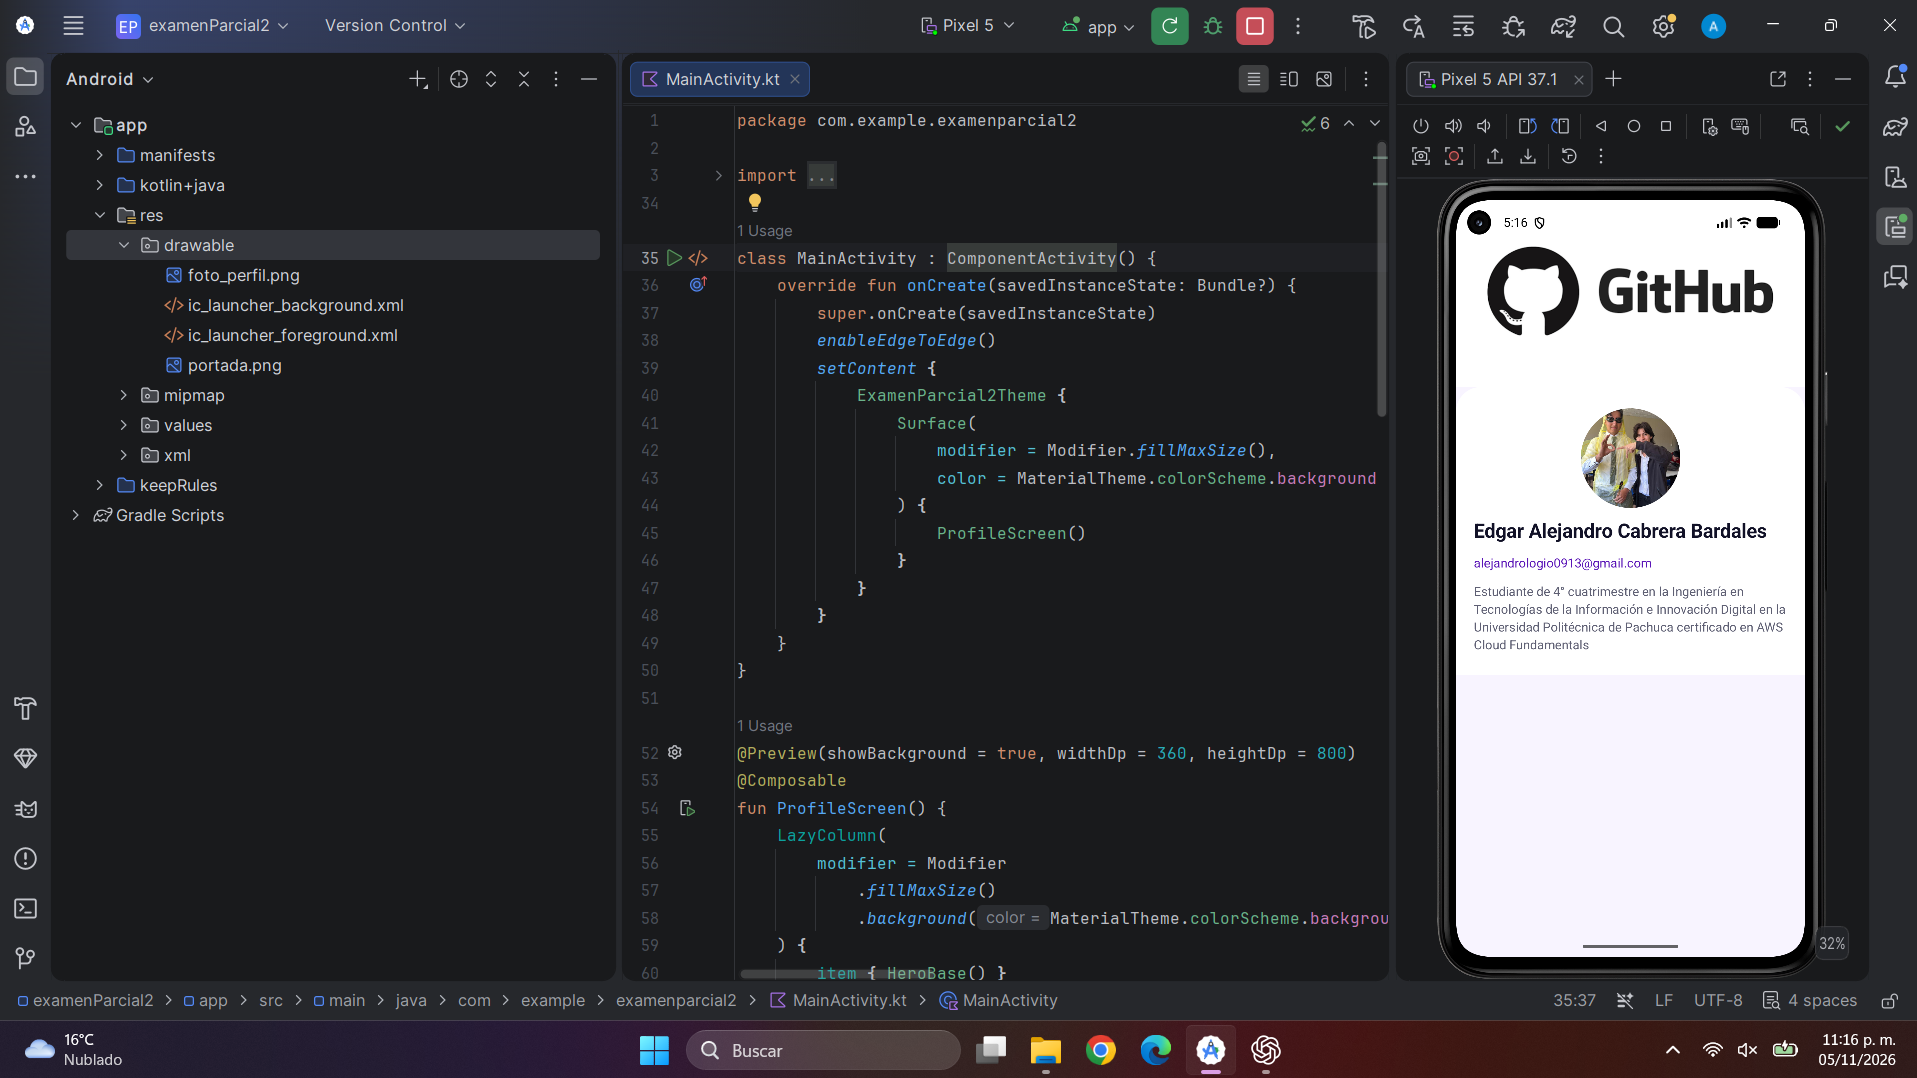
\includegraphics[width=\textwidth]{figura_01.png}
  \caption{Pantalla inicial}
\end{figure}

\subsection{Ajuste de la portada}

Posteriormente, se modifica la función encargada de la portada. La imagen utiliza el ancho disponible y una altura definida para evitar que ocupe toda la pantalla. También se conserva el recorte necesario para que el logotipo permanezca visible dentro del encabezado.

Como se aprecia en la figura 2, la portada ya mantiene una proporción estable y el contenido comienza debajo de ella. Este cambio establece la base sobre la cual se agregarán los elementos superpuestos.

\begin{figure}[H]
  \centering
  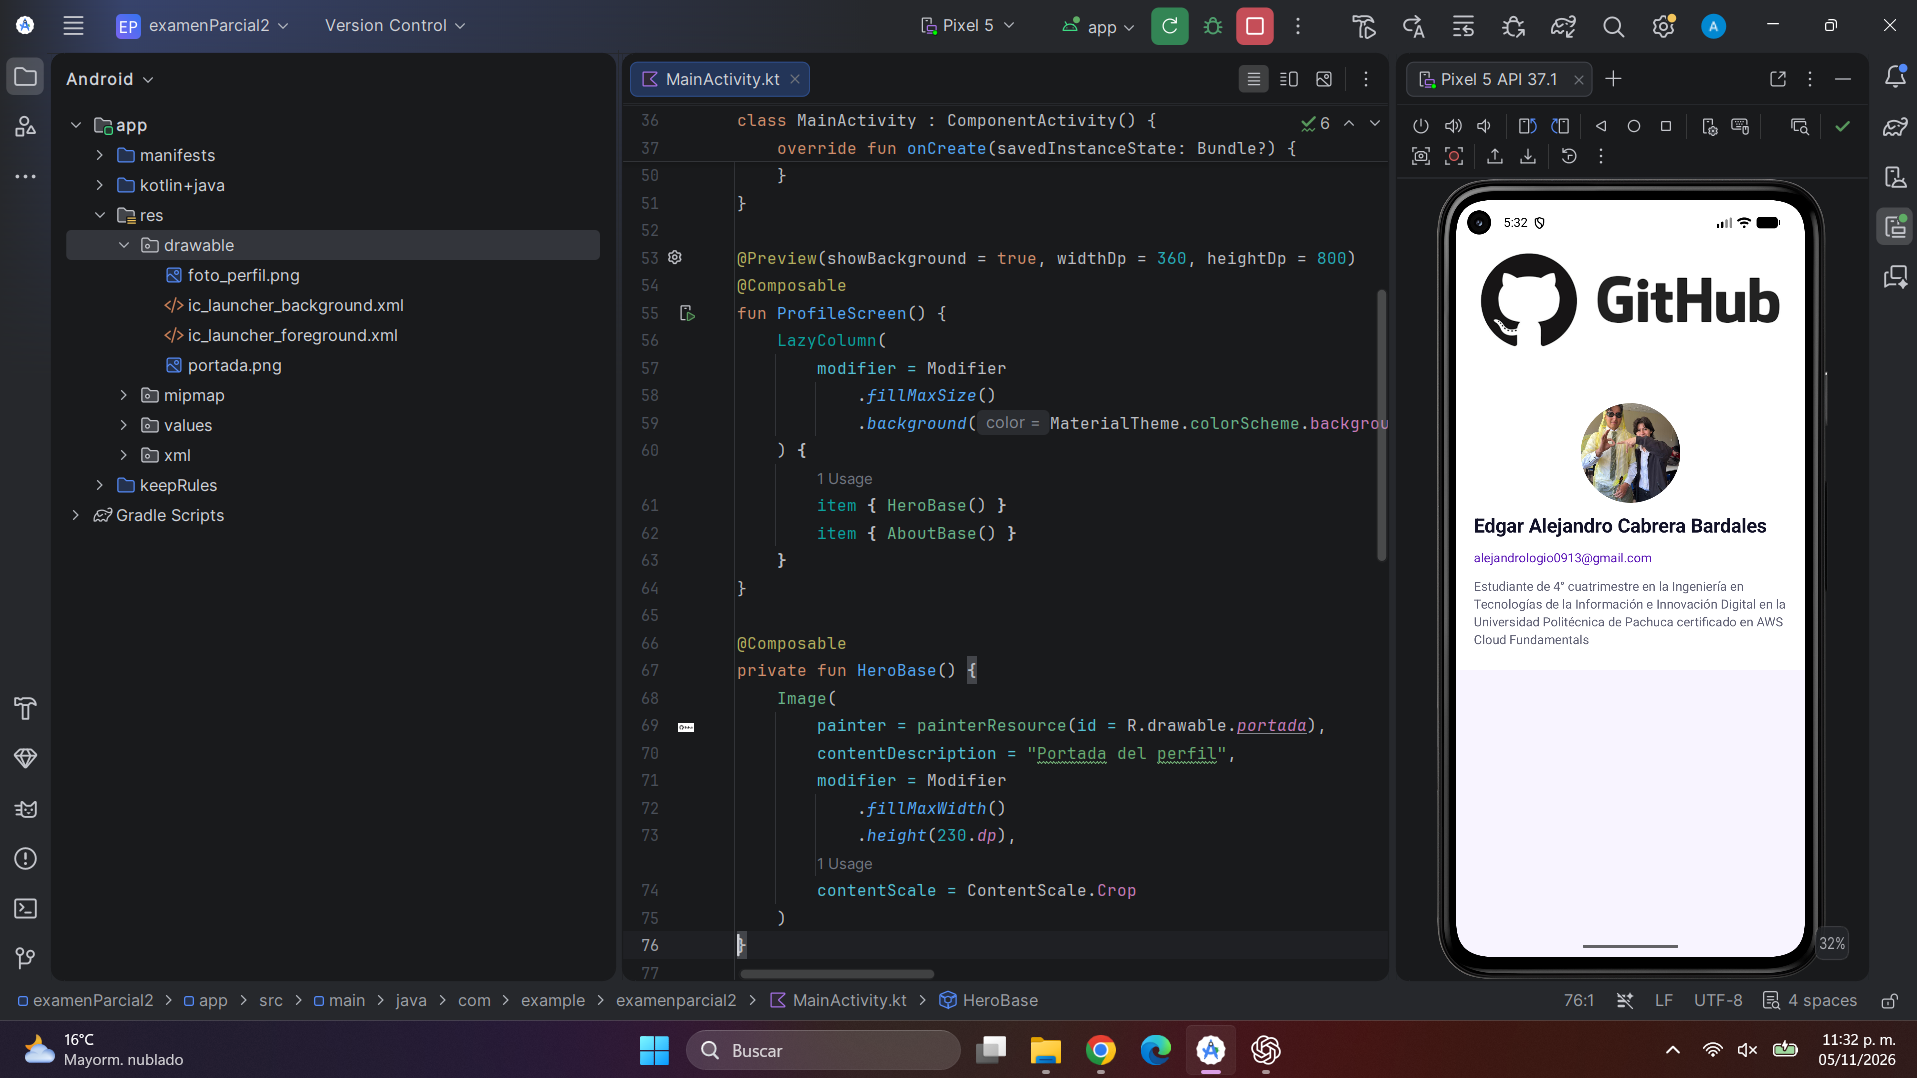
\includegraphics[width=\textwidth]{figura_02.png}
  \caption{Ajuste de portada}
\end{figure}

\subsection{Creación del encabezado superior}

El siguiente paso consiste en agregar acciones sobre la portada. Se crea una etiqueta que identifica a la Universidad Politécnica de Pachuca y se coloca un botón circular para compartir. Ambos elementos se distribuyen en una fila y se separan de la barra de estado del dispositivo.

En la figura 3 podemos observar que la insignia institucional aparece en la parte superior izquierda y el botón de compartir se encuentra a la derecha. Con ello, la portada comienza a presentar una estructura semejante a la referencia visual.

\begin{figure}[H]
  \centering
  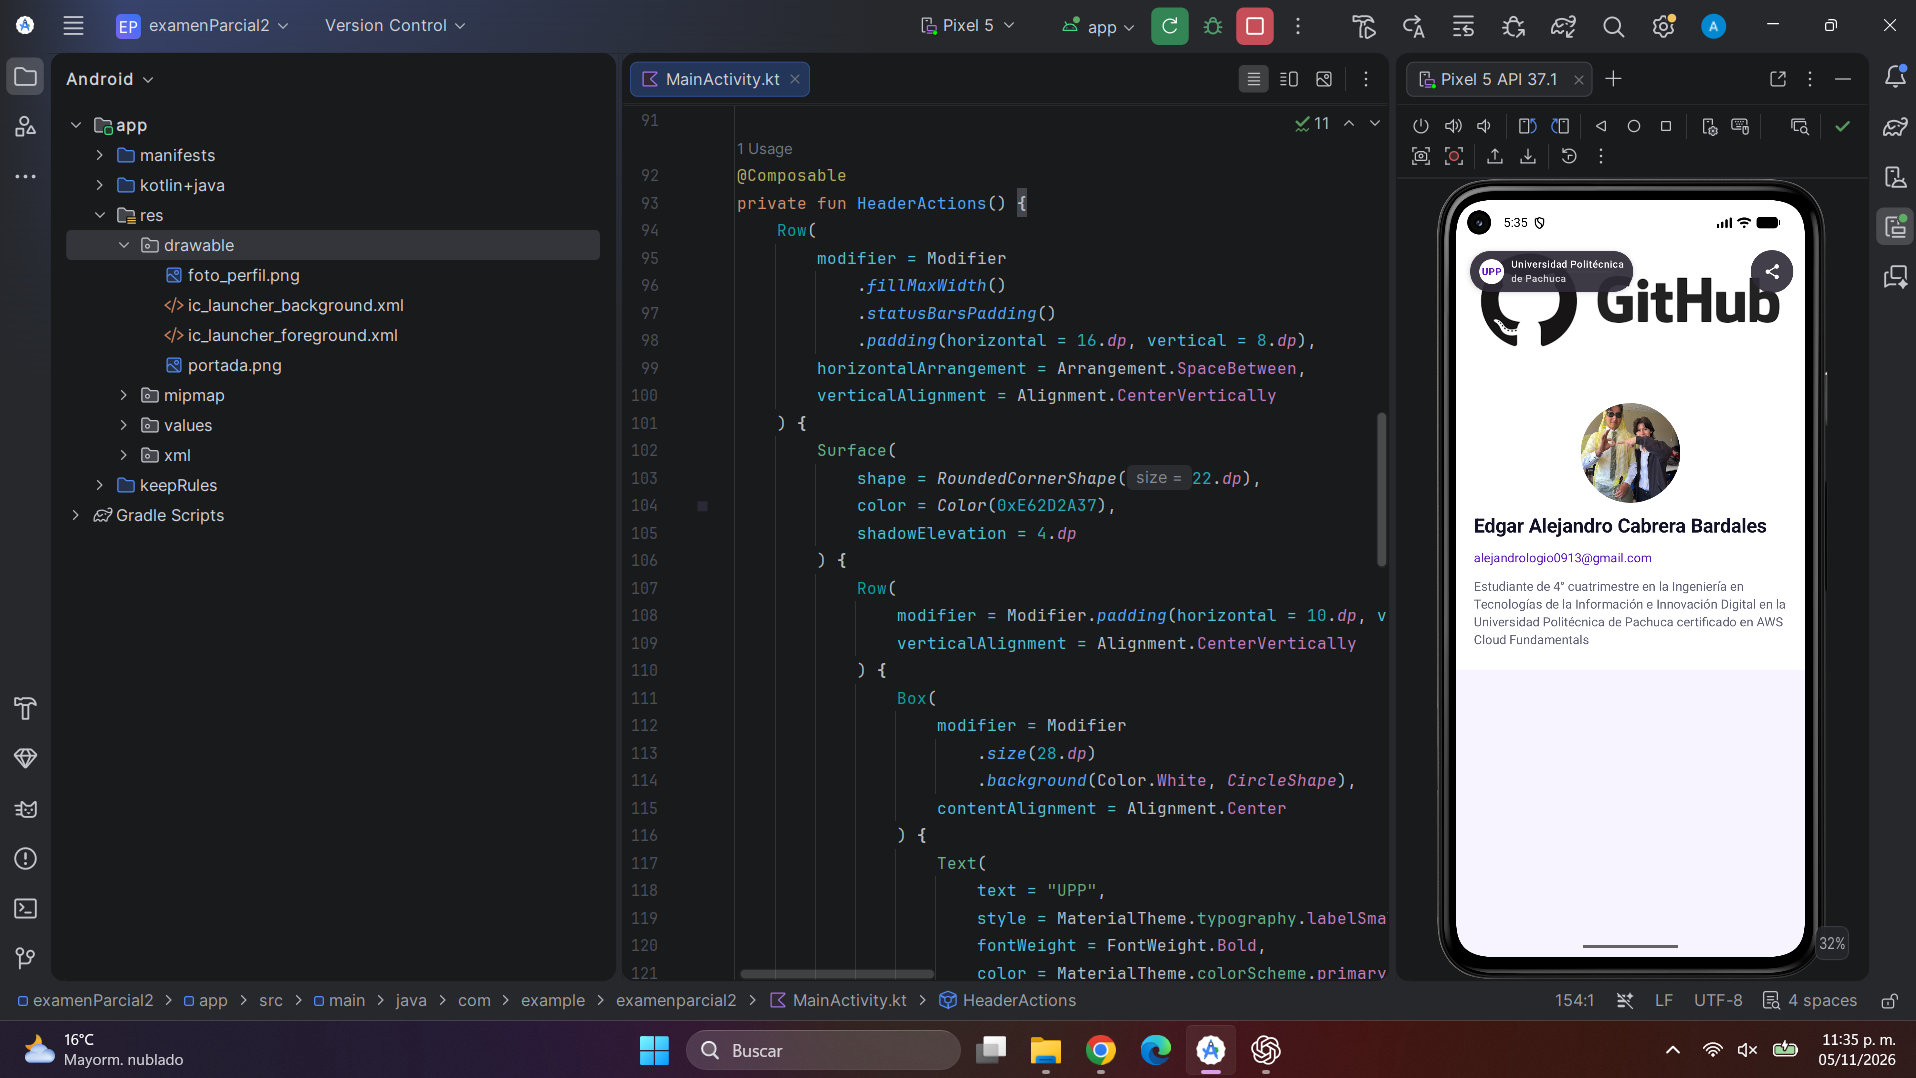
\includegraphics[width=\textwidth]{figura_03.png}
  \caption{Encabezado superior}
\end{figure}

\subsection{Superposición de la fotografía}

Después de construir el encabezado, se reorganiza la fotografía de perfil. Para lograr la superposición se utiliza un contenedor por capas, permitiendo que la imagen sobresalga entre la portada y la sección blanca. La fotografía conserva su forma circular, un borde blanco y un botón pequeño de cámara.

Como podemos observar en la figura 4, la imagen se desplaza hacia la izquierda y deja de aparecer centrada. Este ajuste permite aprovechar mejor el espacio disponible y acercar la pantalla al diseño solicitado.

\begin{figure}[H]
  \centering
  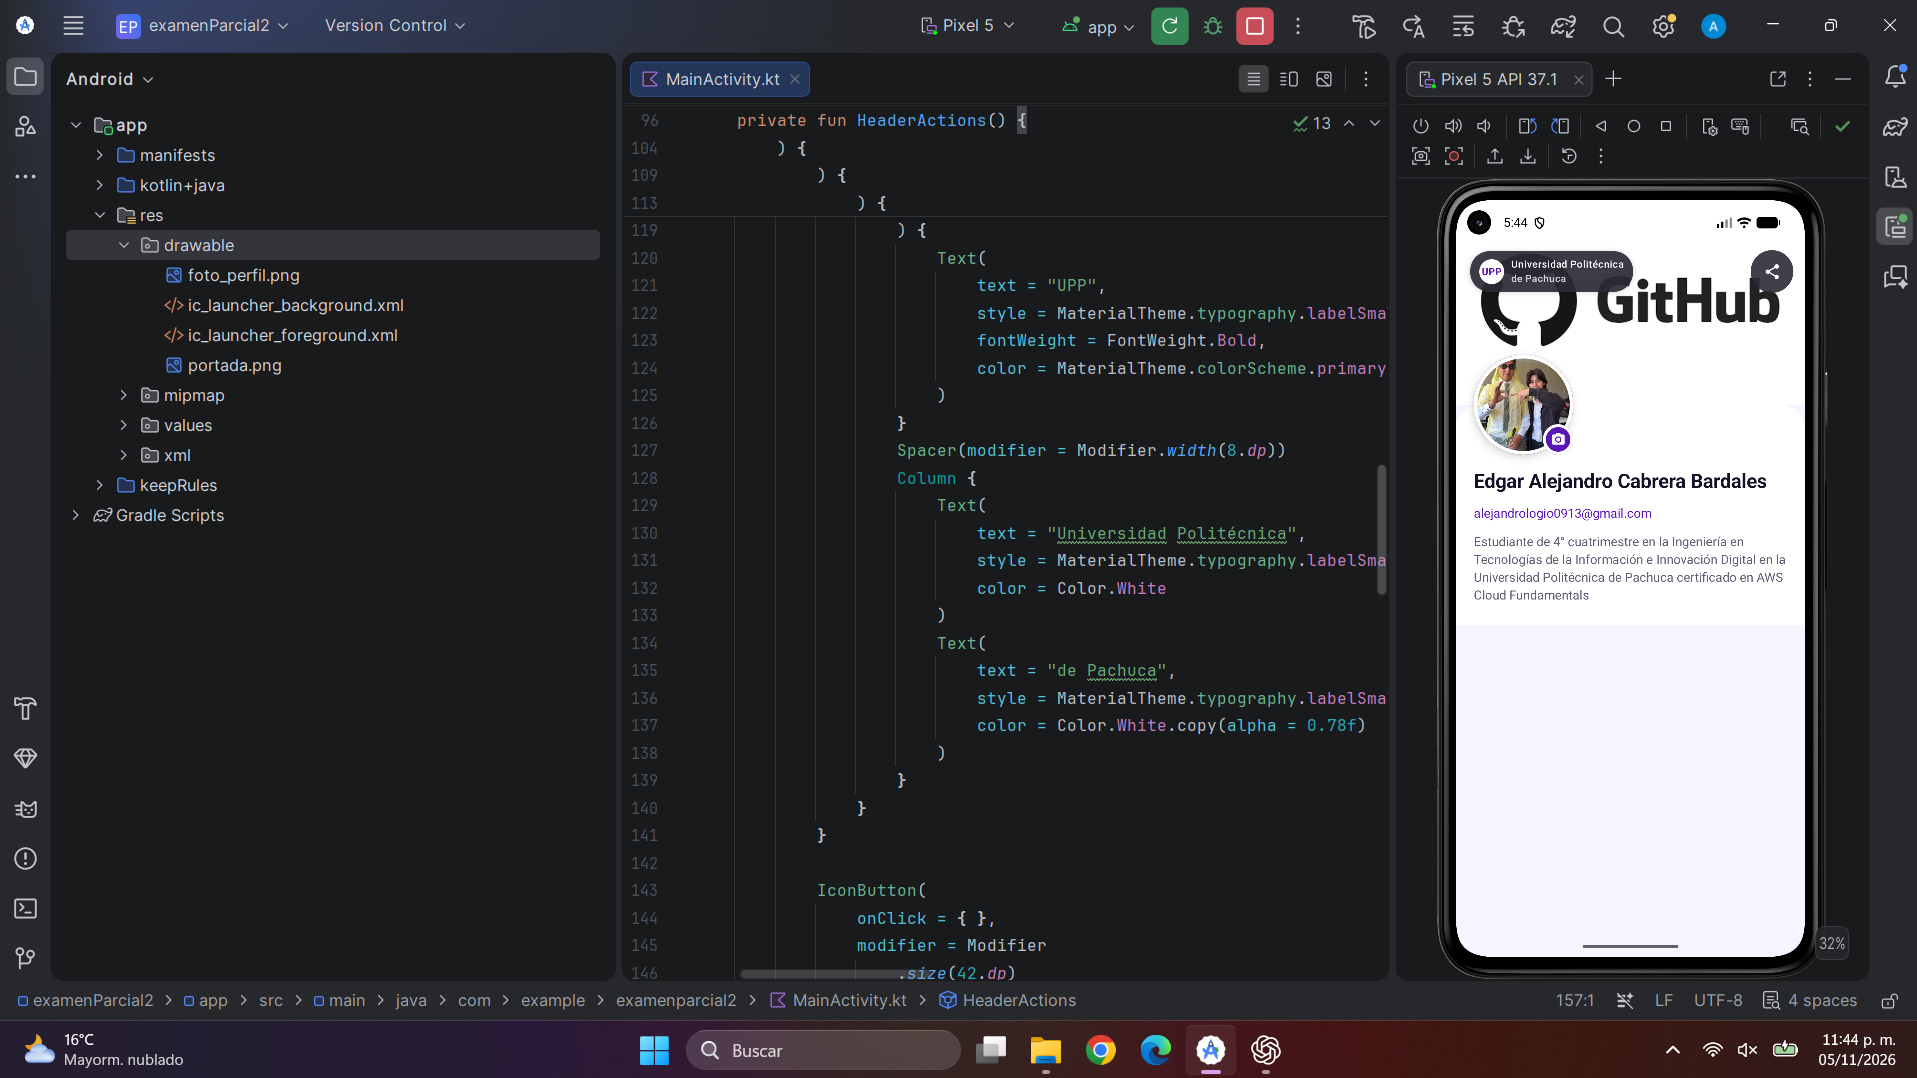
\includegraphics[width=\textwidth]{figura_04.png}
  \caption{Perfil superpuesto}
\end{figure}

\subsection{Organización de los datos personales}

Una vez colocada la fotografía, se mejora la identidad visual del perfil. El nombre se acompaña de una insignia de verificación y se agrega una etiqueta con el texto UPP Software. El correo se mantiene en color morado para distinguirlo de la información general.

En la figura 5 podemos visualizar el bloque correspondiente a la identidad del usuario y el resultado obtenido en el emulador. La información se mantiene legible y relacionada con la fotografía de perfil.

\begin{figure}[H]
  \centering
  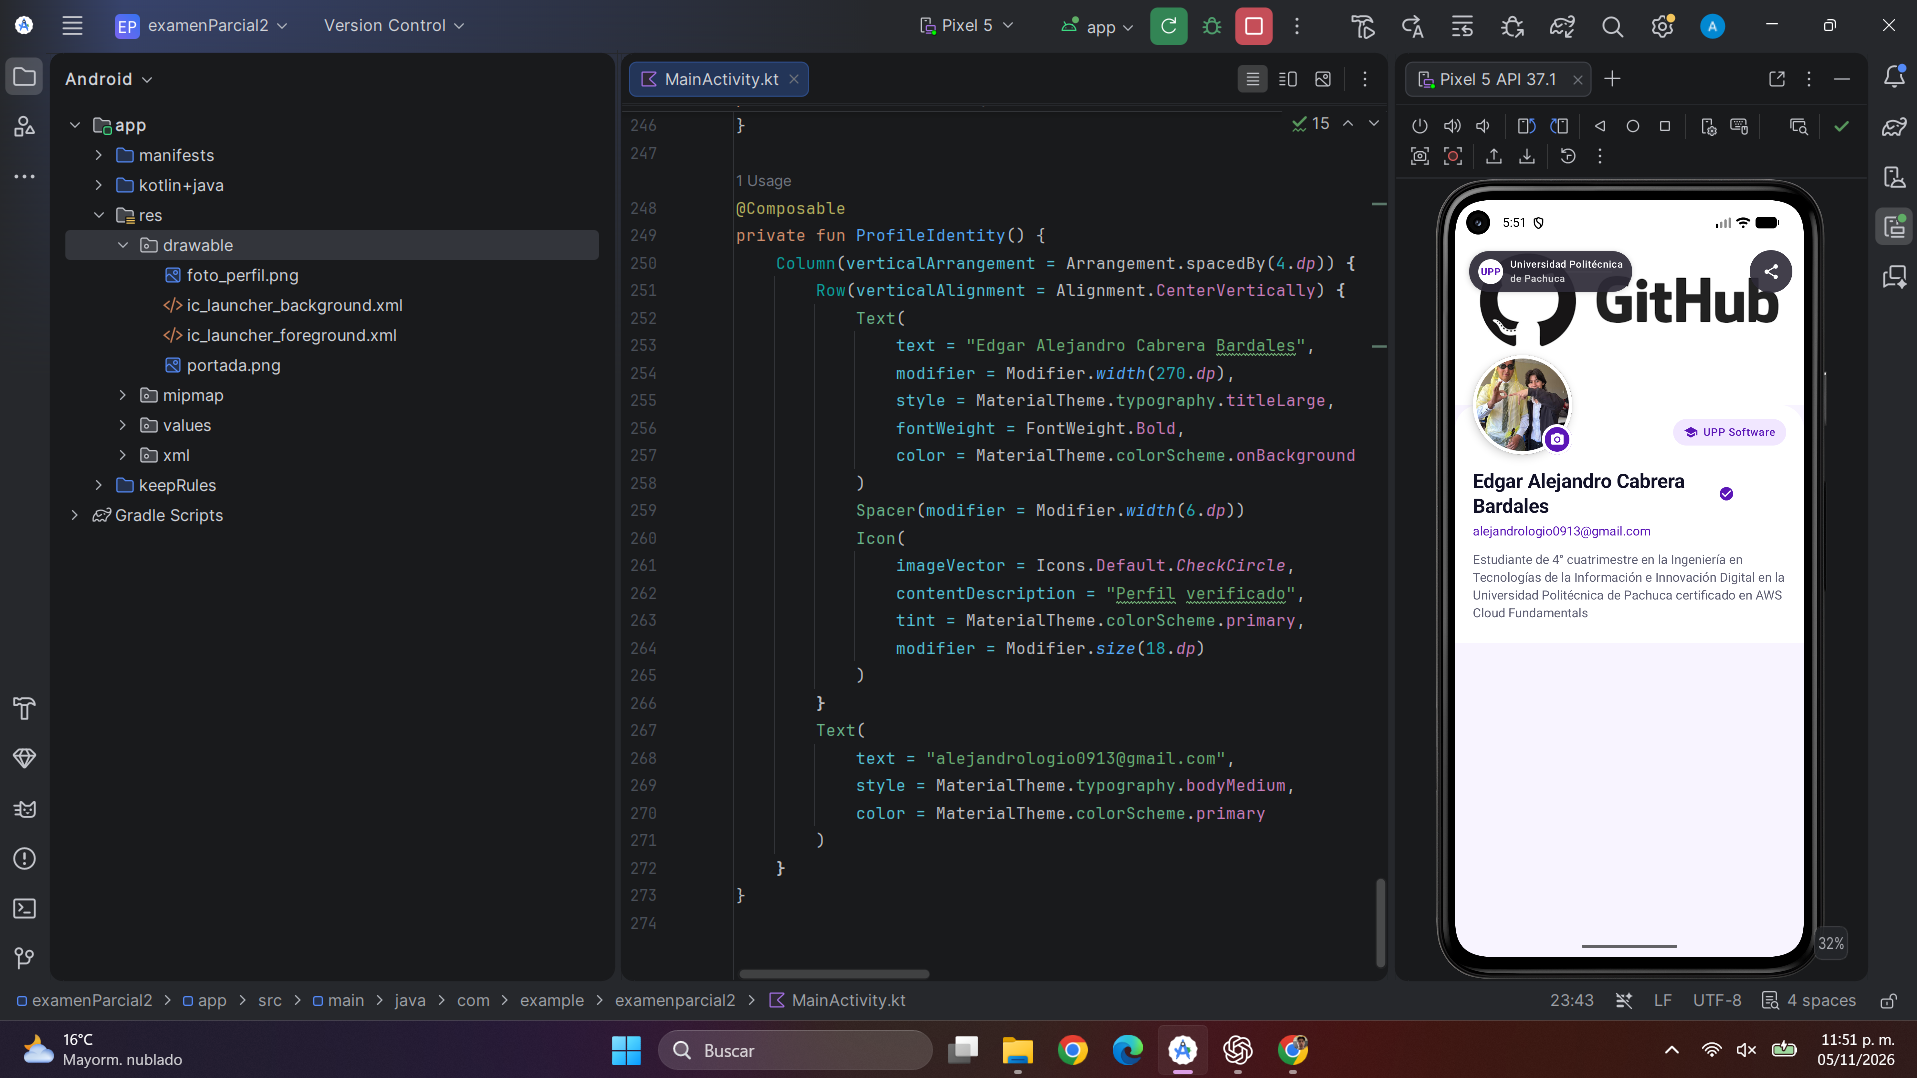
\includegraphics[width=\textwidth]{figura_05.png}
  \caption{Datos del perfil}
\end{figure}

\subsection{Incorporación de la biografía}

Posteriormente, se agrega una sección con el cargo y la descripción personal. El primer texto identifica al usuario como estudiante de tecnologías de la información y desarrollador móvil y web. Debajo se presenta una breve biografía relacionada con el desarrollo de aplicaciones, la innovación digital y los servicios en la nube.

Como se muestra en la figura 6, la función de biografía separa ambos textos y utiliza el color principal para resaltar el cargo. De esta forma, la pantalla presenta la información de manera más clara sin agregar controles innecesarios.

\begin{figure}[H]
  \centering
  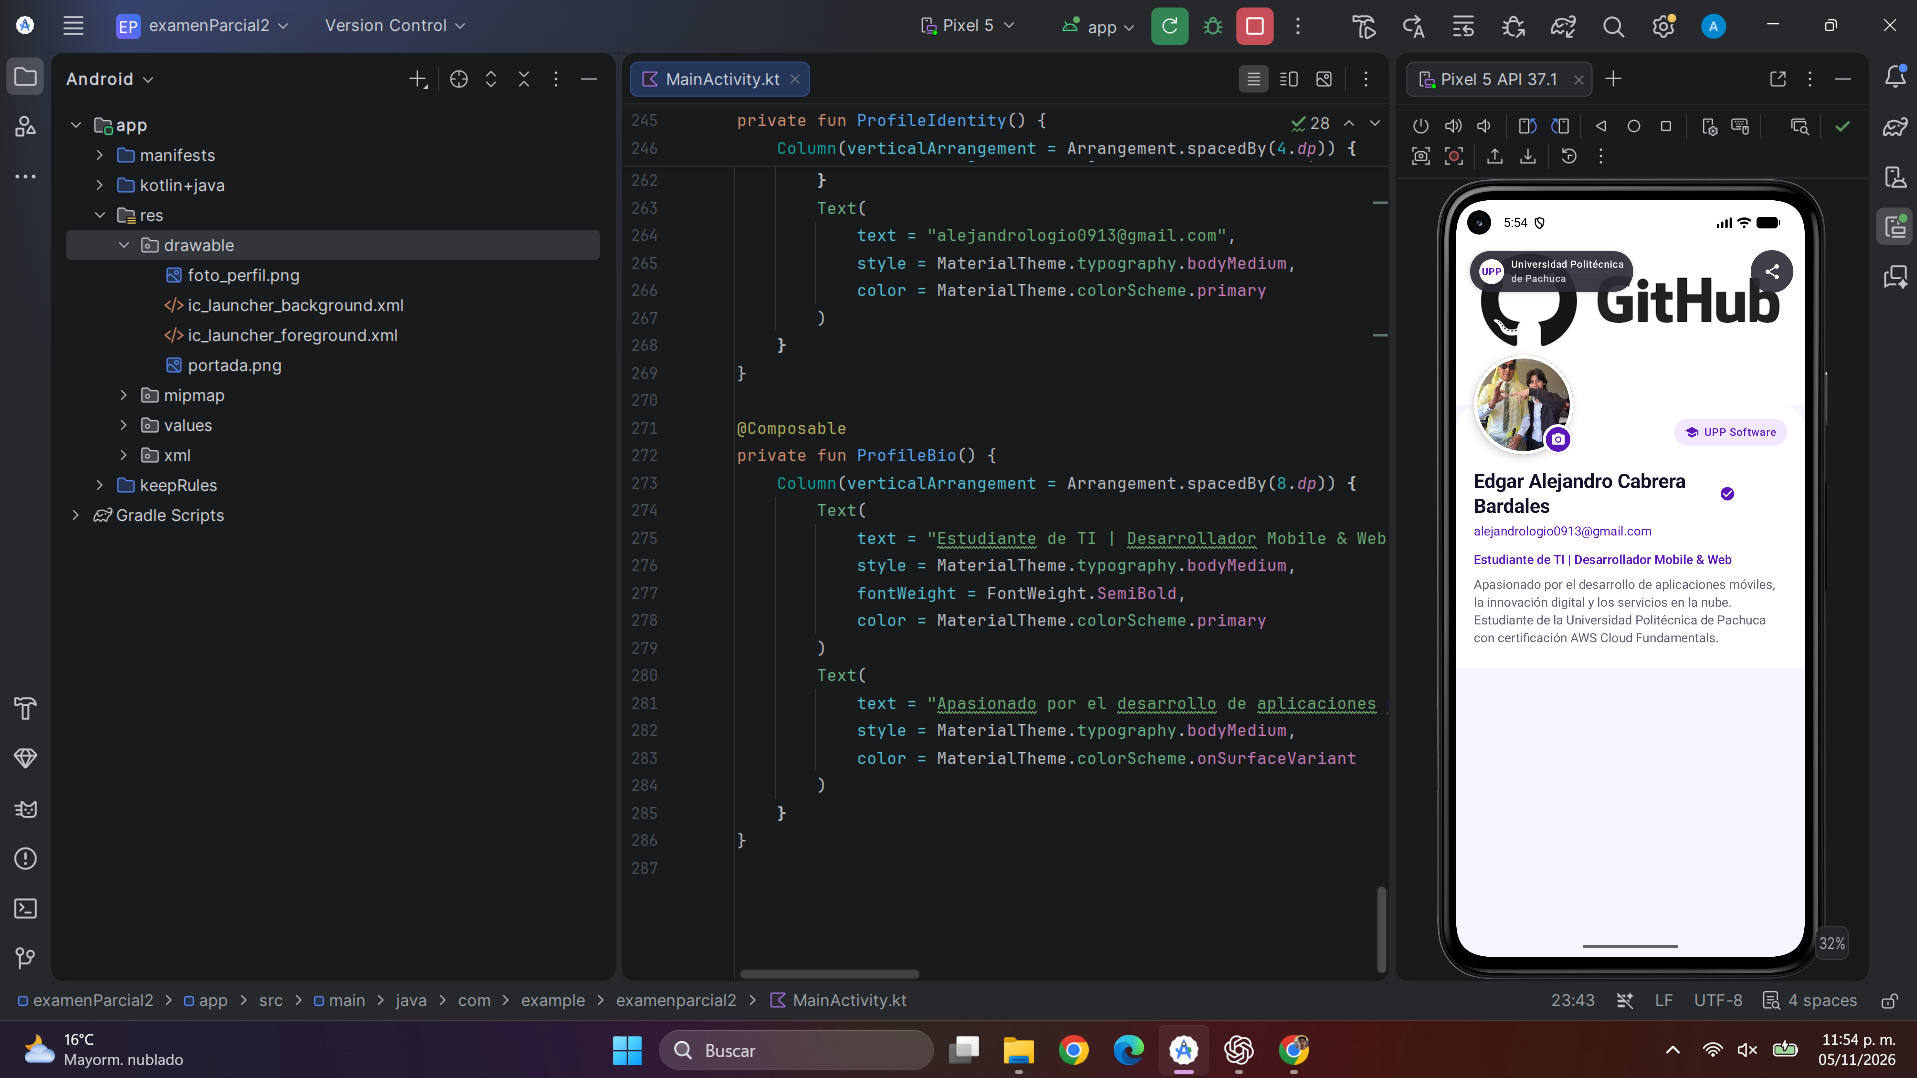
\includegraphics[width=\textwidth]{figura_06.png}
  \caption{Biografía del usuario}
\end{figure}

\subsection{Lista de lenguajes de programación}

El siguiente paso consiste en crear el apartado de lenguajes de programación. Se agrega un encabezado acompañado de la indicación para deslizar y una lista horizontal formada por etiquetas de texto. La lista incluye Kotlin, Java, JavaScript, PHP, C++, C\#, Python y SQL.

En la figura 7 podemos observar que los primeros lenguajes aparecen dentro de etiquetas redondeadas. El desplazamiento horizontal permite consultar los elementos restantes sin aumentar la altura de la pantalla.

\begin{figure}[H]
  \centering
  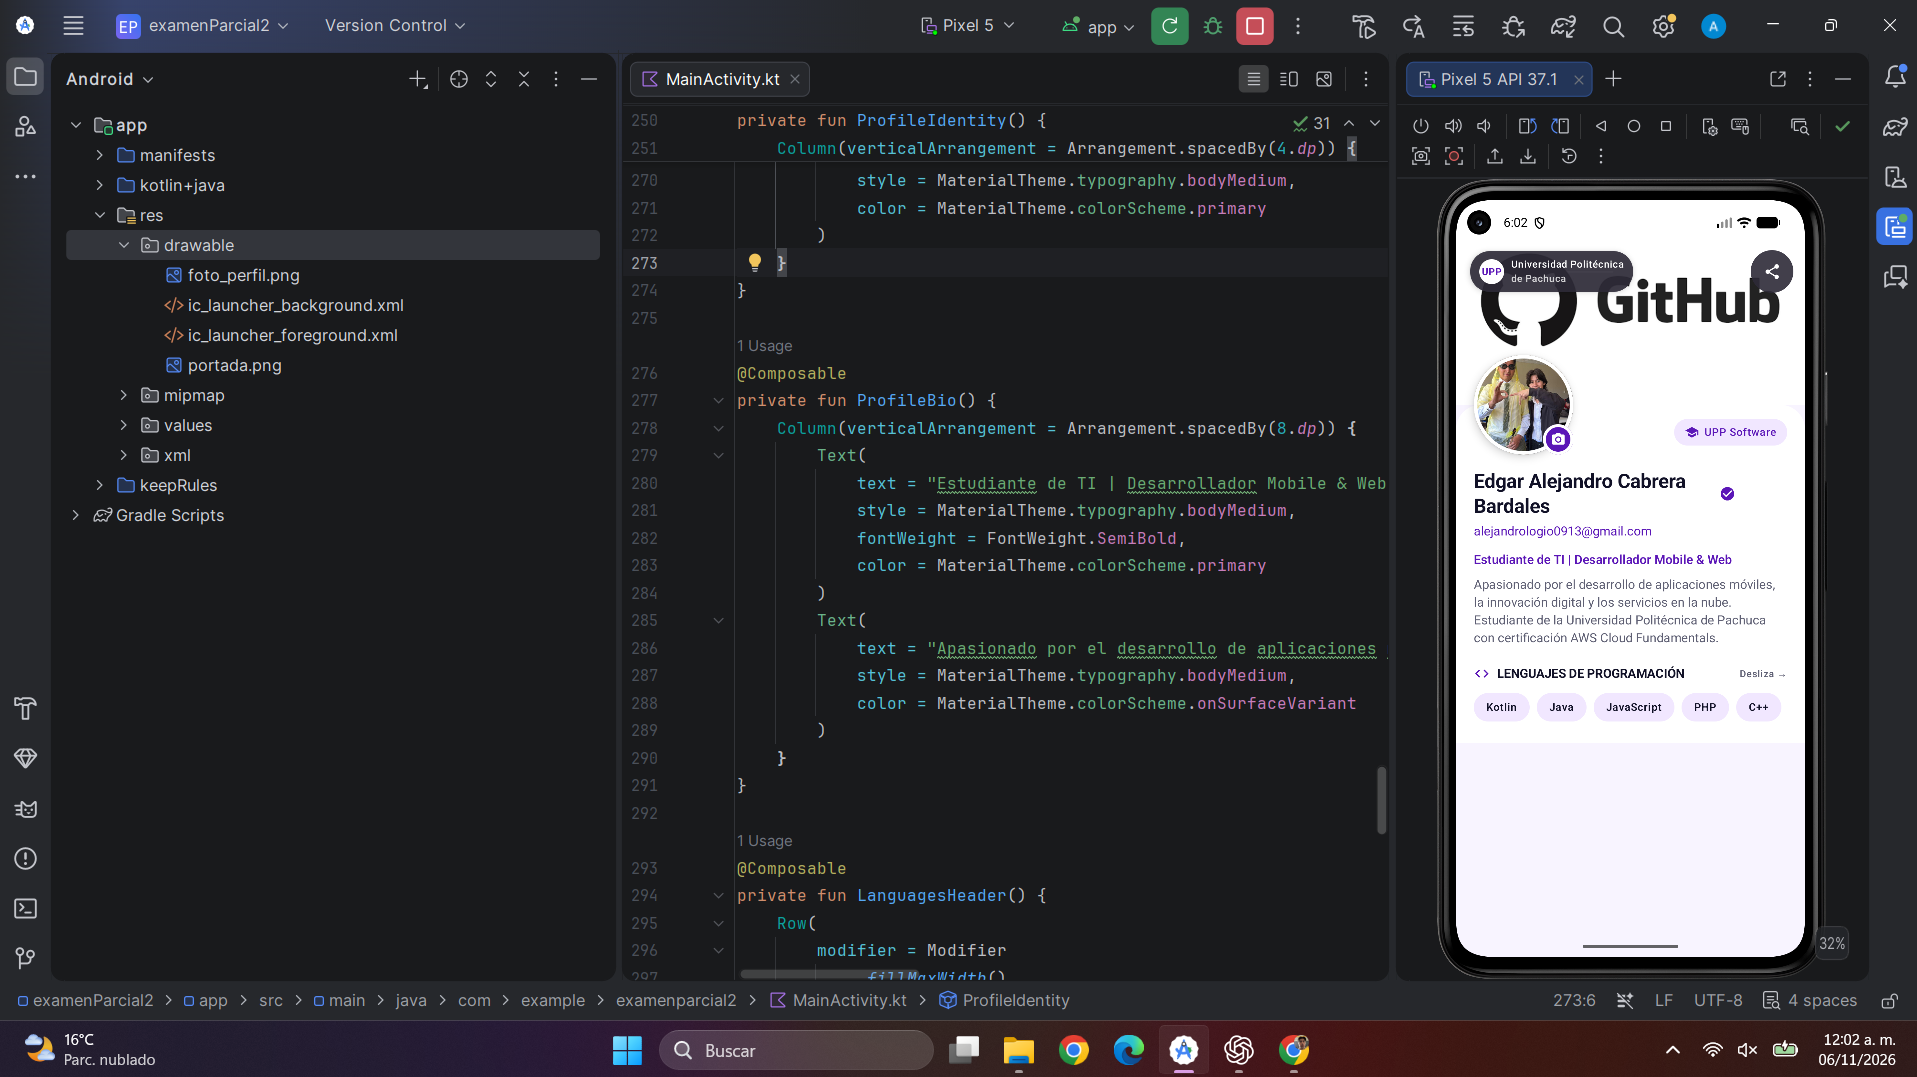
\includegraphics[width=\textwidth]{figura_07.png}
  \caption{Lenguajes agregados}
\end{figure}

\subsection{Configuración de Google Maps}

Para integrar el mapa se agregan las dependencias de Maps Compose y el plugin encargado de administrar la credencial. Posteriormente, el manifiesto recibe la referencia a la clave y se sincroniza el proyecto con Gradle. Por seguridad, el valor de la credencial se mantiene oculto en la evidencia y fuera del código compartido.

Como podemos observar en la figura 8, el mapa se muestra dentro de una tarjeta con esquinas redondeadas en la parte inferior del perfil. Este resultado confirma que la dependencia, el manifiesto y la credencial fueron reconocidos correctamente por la aplicación.

\begin{figure}[H]
  \centering
  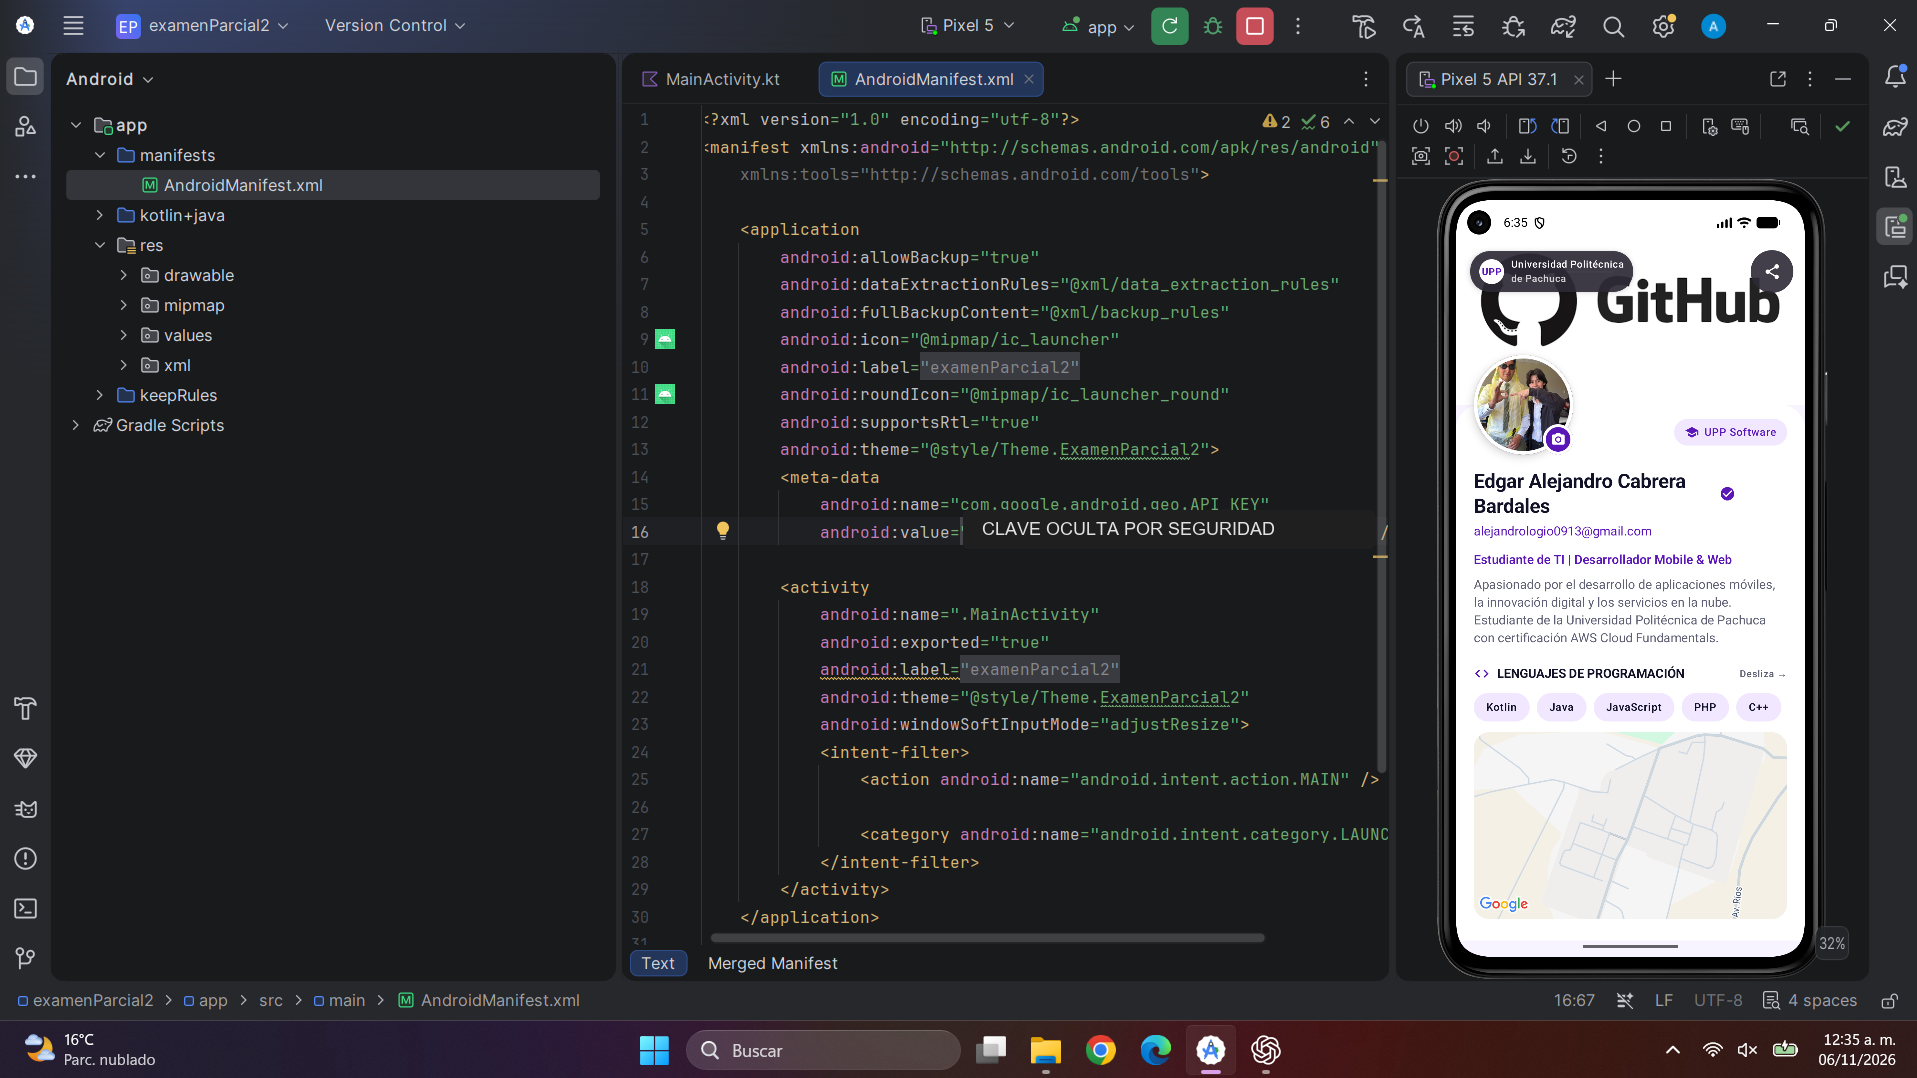
\includegraphics[width=\textwidth]{figura_08.png}
  \caption{Configuración del mapa}
\end{figure}

\subsection{Creación del marcador}

Una vez visible el mapa, se define una ubicación mediante las coordenadas 67.6767 y -67.6767. La cámara se centra en este punto y se coloca un marcador con el título El mejor lugar del mundo. También se agrega una descripción que muestra las coordenadas seleccionadas.

En la figura 9 podemos visualizar el marcador rojo y la ventana informativa abierta. Además, el código muestra la configuración de la cámara, los controles deshabilitados y el contenido asociado al marcador.

\begin{figure}[H]
  \centering
  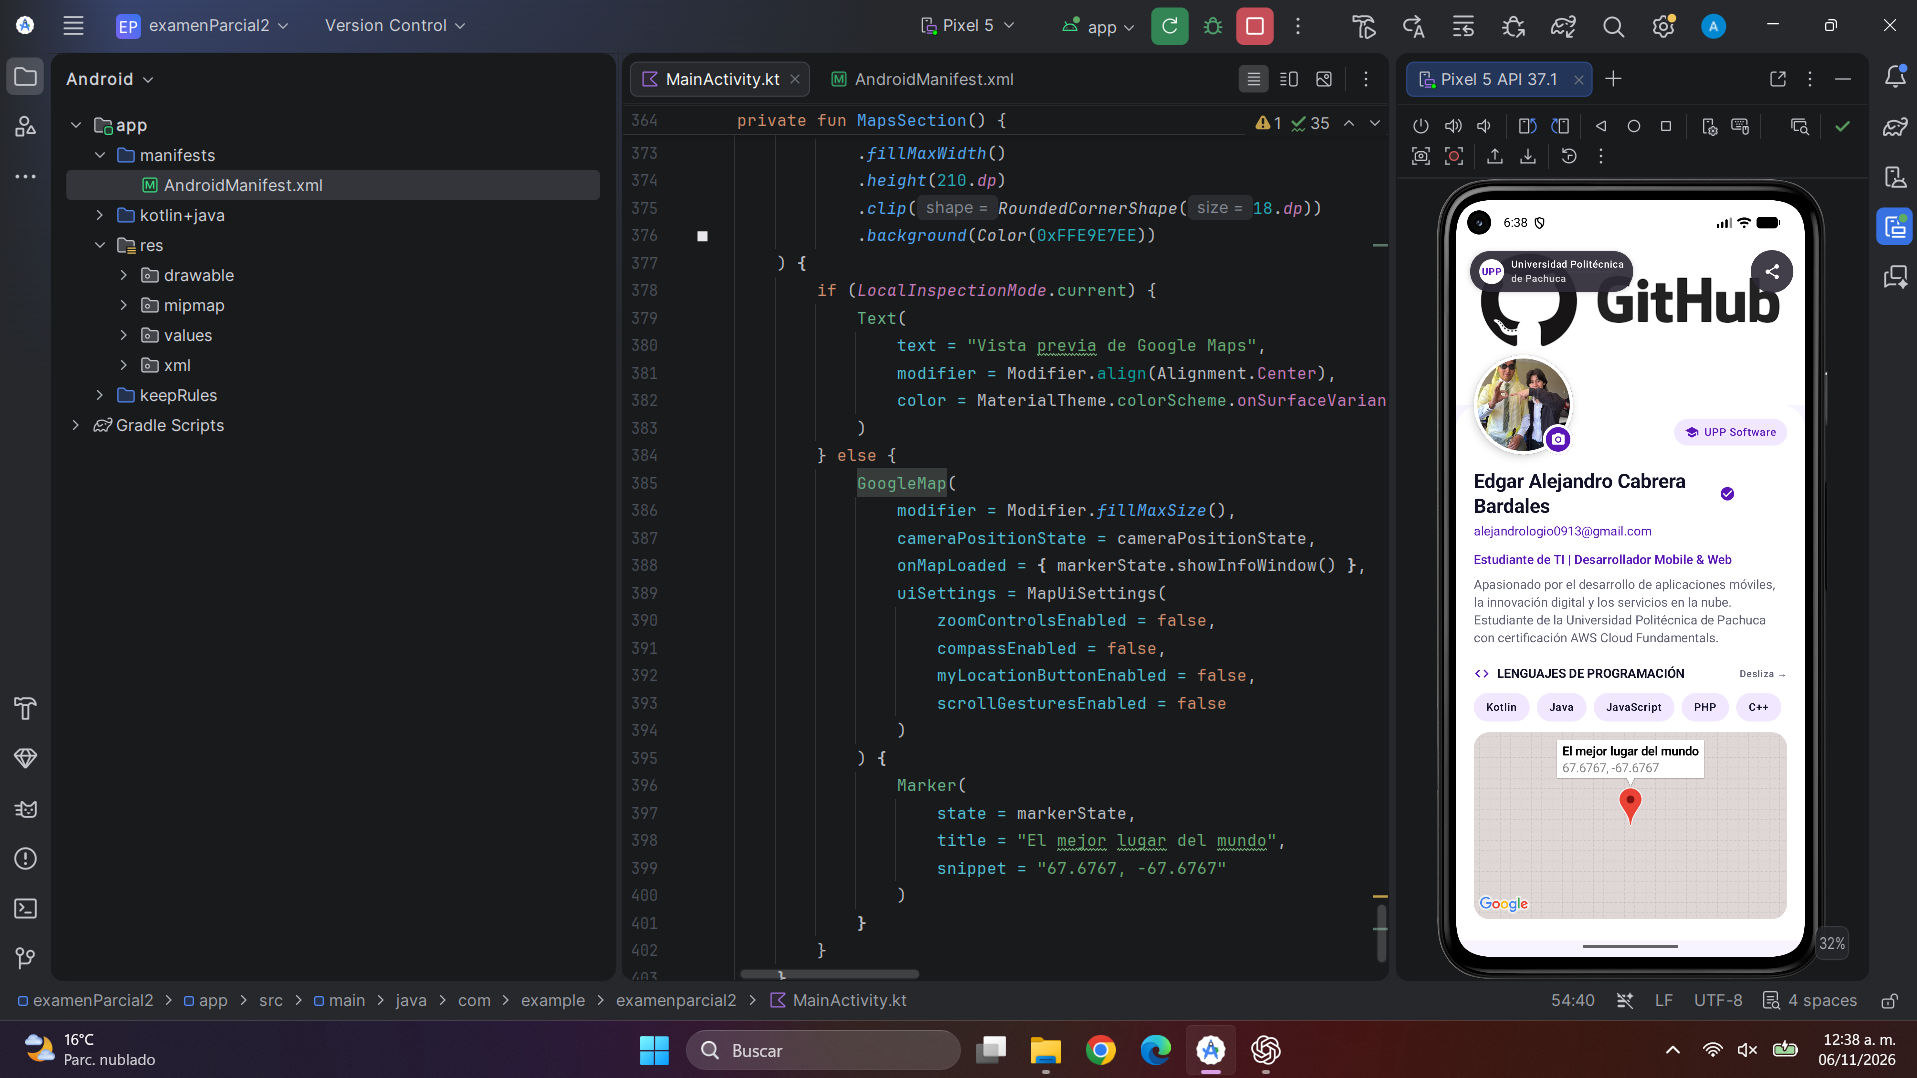
\includegraphics[width=\textwidth]{figura_09.png}
  \caption{Marcador en el mapa}
\end{figure}

\subsection{Implementación del botón flotante}

El siguiente paso consiste en agregar un FloatingActionButton en la esquina inferior derecha. El botón utiliza el color morado principal y presenta un signo más cuando la barra se encuentra cerrada. Su evento de pulsación cambia el valor que controla la visibilidad de la navegación inferior.

Como se aprecia en la figura 10, el botón se muestra sobre el mapa sin impedir el desplazamiento de la pantalla. La evidencia también presenta la variable de estado y la condición utilizada para cambiar el icono del botón.

\begin{figure}[H]
  \centering
  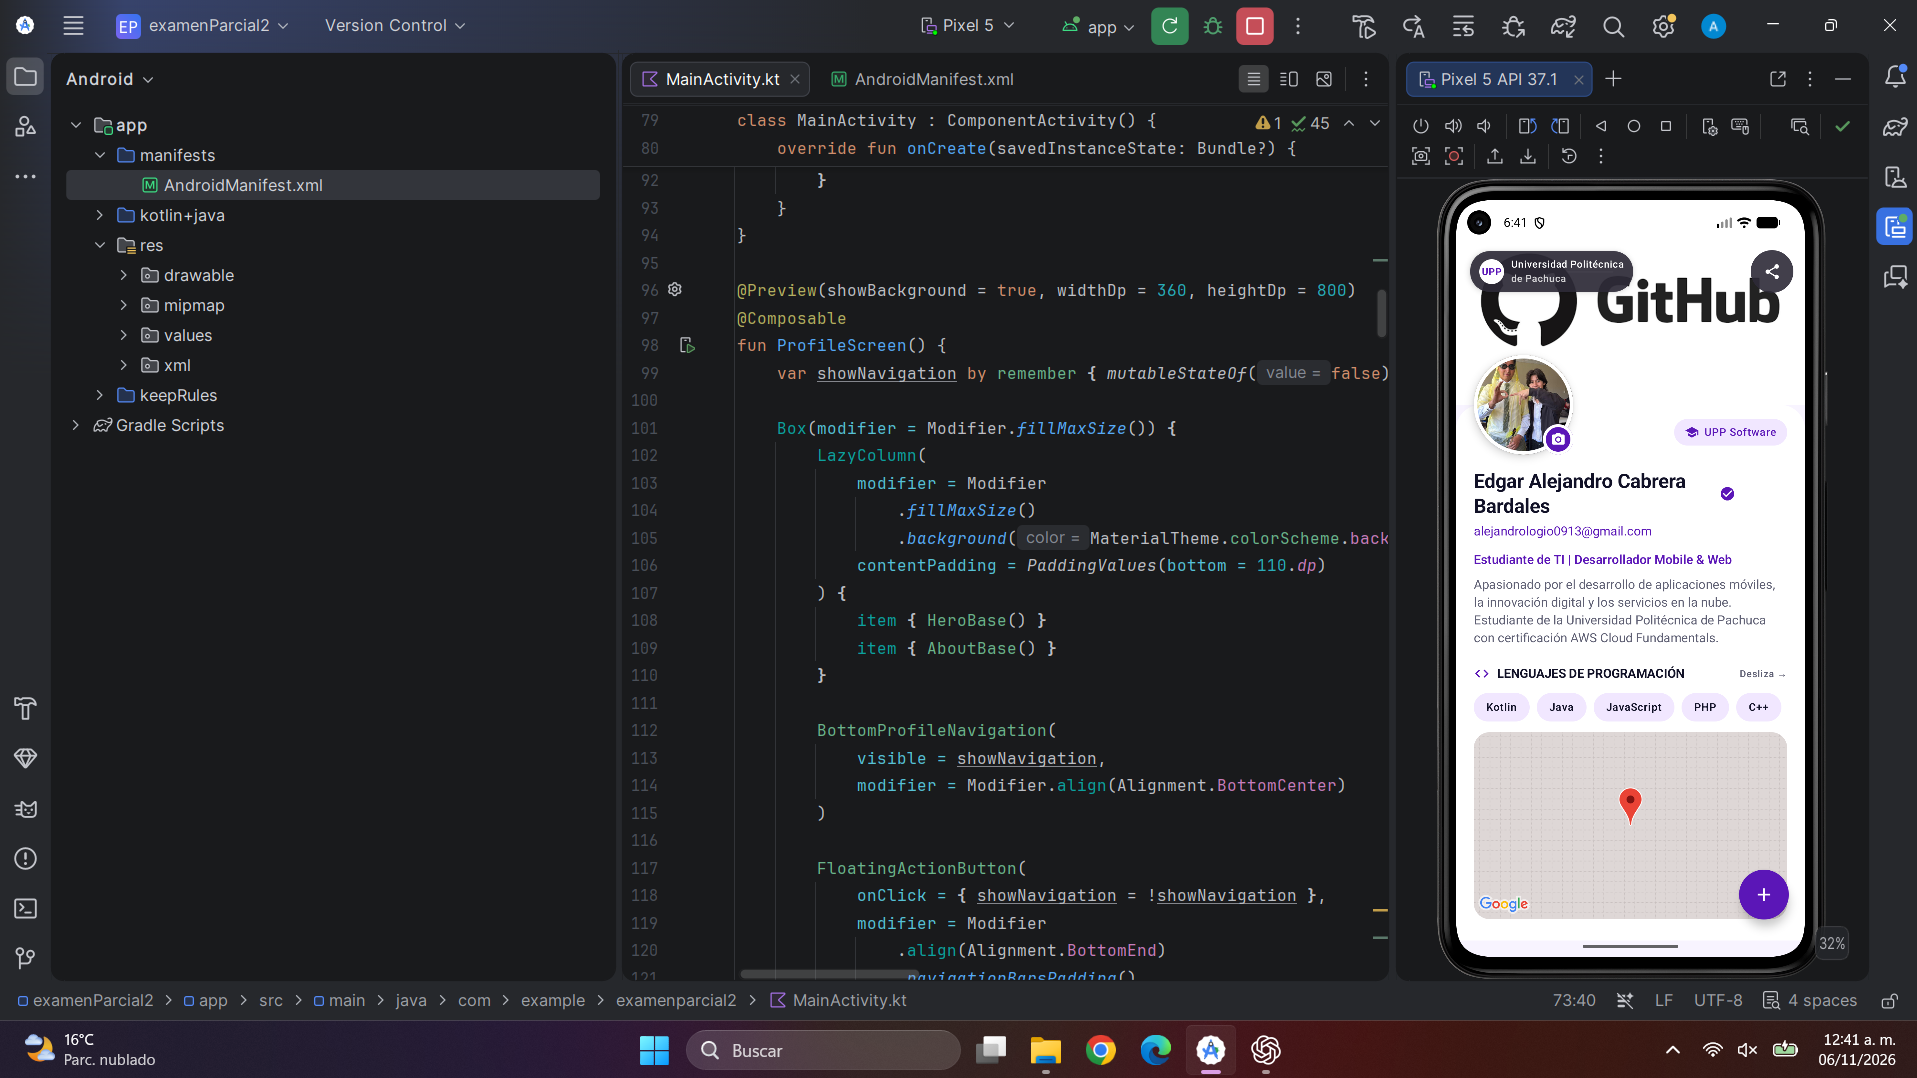
\includegraphics[width=\textwidth]{figura_10.png}
  \caption{Botón flotante}
\end{figure}

\subsection{Despliegue de la barra inferior}

Finalmente, se pulsa el botón flotante para cambiar el estado de la pantalla. AnimatedVisibility muestra una barra inferior con las opciones Inicio, Perfil, Código y Mapa. Estas opciones se agregan como elementos visuales y no realizan navegación hacia otras pantallas, de acuerdo con el alcance solicitado.

En la figura 11 podemos observar la barra desplegada y el cambio del signo más por un icono de cierre. Al pulsar nuevamente el botón, la barra desaparece y la pantalla regresa al estado anterior. Con esta prueba se comprueba que la interfaz final responde correctamente a la interacción.

\begin{figure}[H]
  \centering
  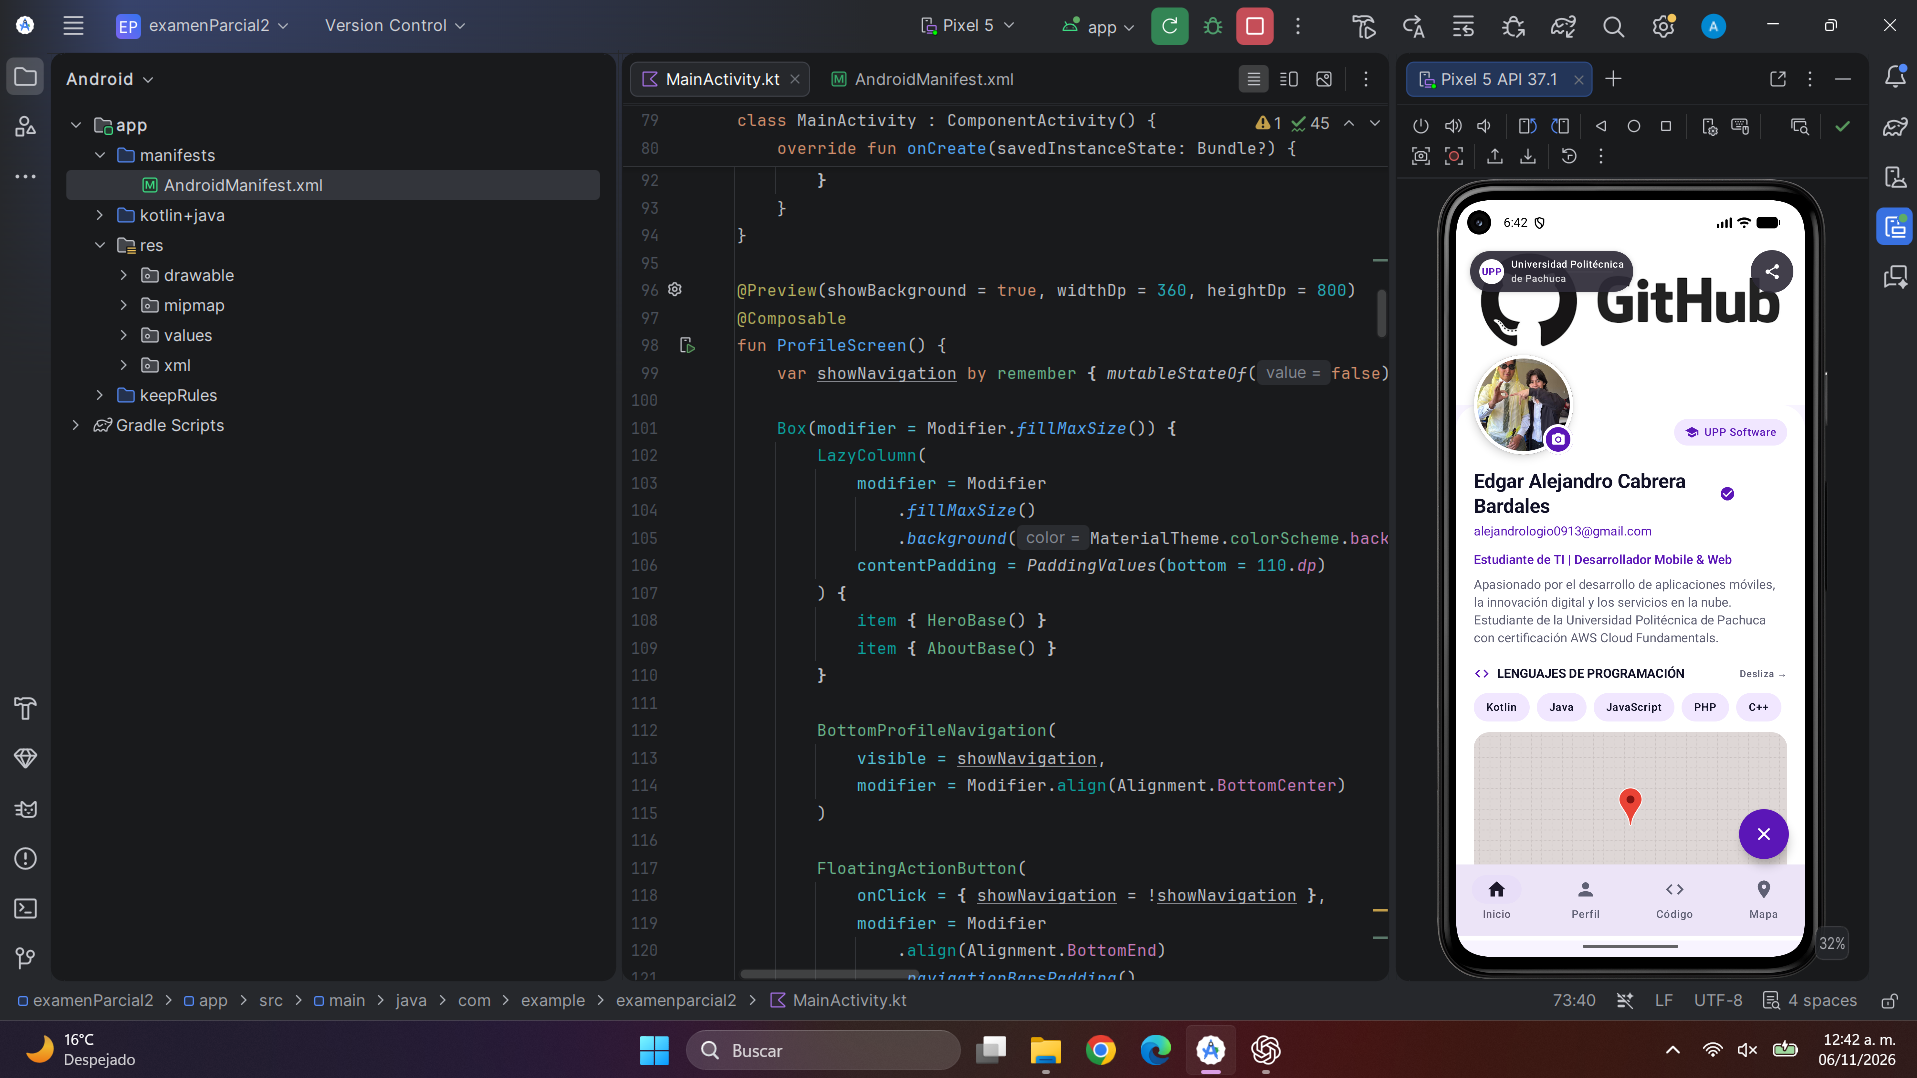
\includegraphics[width=\textwidth]{figura_11.png}
  \caption{Barra inferior desplegada}
\end{figure}

\section{Conclusiones}

El desarrollo de esta práctica permitió transformar una pantalla básica en un perfil profesional completo mediante Jetpack Compose. Se comprobó que los contenedores y modificadores permiten organizar la portada, superponer la fotografía y distribuir textos e iconos sin utilizar archivos XML para la interfaz principal.

Asimismo, LazyColumn y LazyRow facilitaron el desplazamiento vertical de la pantalla y la consulta horizontal de los lenguajes de programación. La integración de Google Maps permitió mostrar un servicio externo dentro de la composición y colocar un marcador con información asociada a coordenadas específicas.

Finalmente, el manejo de estado permitió controlar la visibilidad de la barra inferior desde el botón flotante. La ejecución en el emulador confirmó que el contenido, el mapa, el marcador y la animación de la barra pueden convivir dentro de una misma pantalla sin eliminar los elementos elaborados en etapas anteriores.

\section{Recomendaciones}

Se recomienda mantener las funciones composables separadas de acuerdo con la responsabilidad de cada sección. Esta organización facilita identificar la portada, la identidad, la biografía, los lenguajes, el mapa y la navegación cuando sea necesario realizar una modificación.

También conviene sincronizar y compilar el proyecto después de agregar una dependencia externa, pues una versión incompatible puede producir varios errores simultáneos en Android Studio. En el caso de Google Maps, la clave debe mantenerse en un archivo excluido del control de versiones y restringirse al paquete y certificado de la aplicación.

Por último, se recomienda ejecutar las interacciones en un emulador o dispositivo real. La vista previa permite revisar la distribución general, pero no sustituye la comprobación del mapa, el marcador, el desplazamiento y la animación de la barra inferior.

\clearpage
\section{Anexo}
\vfill
\clearpage
\section{Referencias}

\setstretch{1.5}
\setlength{\parindent}{0pt}

Android Developers. (2026a). \textit{Compose layout basics}. Google.\\
\url{https://developer.android.com/develop/ui/compose/layouts/basics}

Android Developers. (2026b). \textit{Lazy lists and lazy grids}. Google.\\
\url{https://developer.android.com/develop/ui/compose/lists}

Android Developers. (2026c). \textit{State and Jetpack Compose}. Google.\\
\url{https://developer.android.com/develop/ui/compose/state}

Android Developers. (2026d). \textit{Floating action button}. Google.\\
\url{https://developer.android.com/develop/ui/compose/components/fab}

Android Developers. (2026e). \textit{Animation modifiers and composables}. Google.\\
\url{https://developer.android.com/develop/ui/compose/animation/composables-modifiers}

Android Developers. (2026f). \textit{Navigation bar}. Google.\\
\url{https://developer.android.com/develop/ui/compose/components/navigation-bar}

Google Maps Platform. (2026a). \textit{Maps Compose Library}. Google.\\
\url{https://developers.google.com/maps/documentation/android-sdk/maps-compose}

Google Maps Platform. (2026b). \textit{Set up an Android Studio project}. Google.\\
\url{https://developers.google.com/maps/documentation/android-sdk/config}

\end{document}
